\section{Markov chain}

\begin{definition}[\textit{Discrete stochastic process}]
    A discrete stochastic process is a stochastic process that characterizes the stochastic evolution of a system at distinct and separate time steps.
\end{definition}
\begin{definition}[\textit{Continuous stochastic process}]
    A continuous stochastic process is a stochastic process in which the system's state can be observed at any continuous point in time.
\end{definition}
\begin{definition}[\textit{Markov chain}]
    A discrete stochastic process is a first-order Markov chain when, for all $t$ and for all $N$ states, the following condition holds:    \[\Pr\left(X_t\mid X_{t-1},X_{t-2},\dots,X_0\right)=\Pr(X_t\mid X_{t-1})\] 
\end{definition}
\begin{definition}[\textit{Stationary Markov chain}]
    A stationary Markov chain is a Markov chain where the probability of an event is independent of time, expressed as:
    \[\Pr\left(X_{t+1=j}\mid X_t=j\right)=p_{ij}\] 
\end{definition}

A Markov chain can be represented by a transition matrix, where $p_{ij}$ denotes the probability of transitioning from state $i$ to state $j$. 
Alternatively, this transition matrix can be illustrated using a directed graph.

For a Markov chain in state $i$ at time $m$, the probability of being in state $j$ after $n$ steps is given by:
\[\Pr_{ij}(n)=ij^{th} \textnormal{ element of the modified tranisiton matrix }P^n\]
The probability of occupying state $j$ at time $n$, without knowing the exact state of the Markov chain at time 0, is expressed as:
\[\sum_i q_i\cdot\Pr_{ij}(n)=1 \cdot (\textnormal{ column } j \textnormal{ of }P^n) \]
Here, $q_i$ represents the initial state probabilities at time 0.
\begin{example}
    Consider a market with just two brands of Cola. 
    A person buying Cola1 will buy Cola1 again with a probability of 0.9. 
    A person buying Cola2 will buy Cola2 again with a probability of 0.8. 
    The associated transition matrix is:
    \[P=
    \begin{bmatrix}
        0.9 & 0.1 \\
        0.2 & 0.8
    \end{bmatrix}\]
    The corresponding directed graph is shown below:
    \begin{figure}[H]
        \centering
        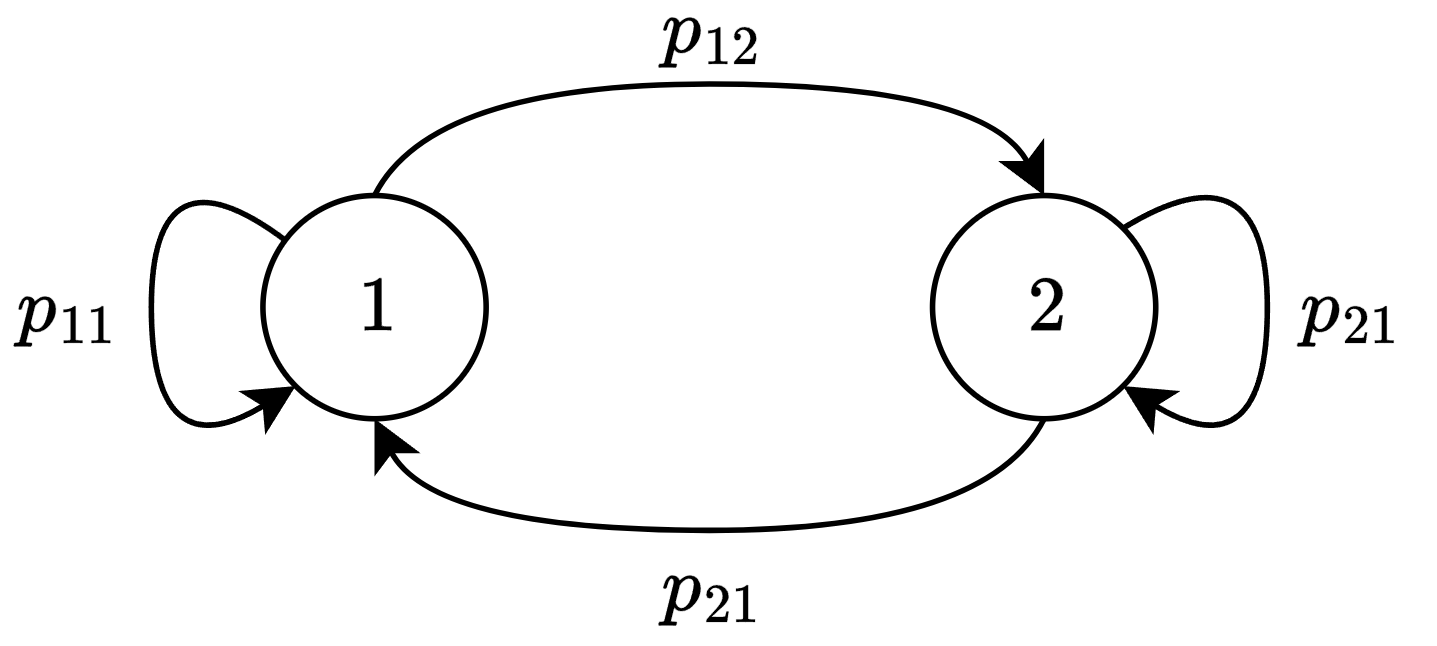
\includegraphics[width=0.5\linewidth]{images/cola.png}
    \end{figure}
    Suppose someone bought Cola2; we want to compute the probability of buying Cola1 after two time steps. 
    To achieve this, we multiply the transition matrix by itself:
    \[P^2=
    \begin{bmatrix}
        0.9 & 0.1 \\
        0.2 & 0.8
    \end{bmatrix}
    \begin{bmatrix}
        0.9 & 0.1 \\
        0.2 & 0.8
    \end{bmatrix}
    =
    \begin{bmatrix}
        0.83 & 0.17 \\
        0.34 & 0.66
    \end{bmatrix}\]
    The desired probability is given by the element in position $p_{12}$ in $P^2$, which is 0.34.
    
    Now, if someone bought Cola1, we want to compute the probability of buying Cola1 after three time steps:
    \[P^3=
    \begin{bmatrix}
        0.9 & 0.1 \\
        0.2 & 0.8
    \end{bmatrix}
    \begin{bmatrix}
        0.9 & 0.1 \\
        0.2 & 0.8
    \end{bmatrix}
    \begin{bmatrix}
        0.9 & 0.1 \\
        0.2 & 0.8
    \end{bmatrix}
    =
    \begin{bmatrix}
        0.781 & 0.219 \\
        0.438 & 0.562
    \end{bmatrix}\]
    The desired probability is given by the element in position $p_{11}$ in $P^3$, which is 0.781.

    If, at some time, 60\% of clients bought Cola1 and 40\% bought Cola2, we want to determine the percentage of people buying Cola1 after three time steps:
    \begin{align*}
        \sum_i q_i \cdot P^3_{ij}   &= q \cdot \left( \textnormal{column } 1 \textnormal{ of }P^3\right) \\
                                    &= \begin{bmatrix} 0.6 & 0.4 \end{bmatrix} \begin{bmatrix} 0.781 \\ 0.438 \end{bmatrix}=0.6438
    \end{align*}
\end{example}
\begin{definition}[\textit{k-th Markov chain}]
    In a $k$-th order Markov chain, each state transition depends on the previous $k$ states.
\end{definition}
\begin{definition}[\textit{Reachable state}]
    The state $j$ is said to be reachable from $i$ if there exists a path from $i$ to $j$.
\end{definition}
\begin{definition}[\textit{Communicating states}]
    The states $i$ and $j$ are said to be communicating if $i$ is reachable from $j$ and vice versa.
\end{definition}
\begin{definition}[\textit{Closed set of states}]
    A set of states $S$ is closed if no state outside $S$ is reachable from a state in $S$.
\end{definition}
\begin{definition}[\textit{Absorbing state}]
    A state $i$ is an absorbing state if $p_{ij} = 1$.
\end{definition}
\begin{definition}[\textit{Transient state}]
    A state $i$ is transient if there exists $j$ reachable from $i$, but $i$ is not reachable from $j$.
\end{definition}
\begin{definition}[\textit{Recurrent state}]
    A state that is not transient is defined as recurrent.
\end{definition}
\begin{definition}[\textit{Periodic state}]
    A state $i$ is periodic with period $k > 1$ if $k$ is the largest number that divides the length of all paths from $i$ to $i$; a state that is not periodic is said to be aperiodic.
\end{definition}
\begin{definition}[\textit{Ergodic}]
    If all states in a Markov chain are recurrent, aperiodic, and communicate with each other, it is said to be ergodic.
\end{definition}
\begin{example}
    Consider the following graphs: 
    \begin{figure}[H]
        \centering
        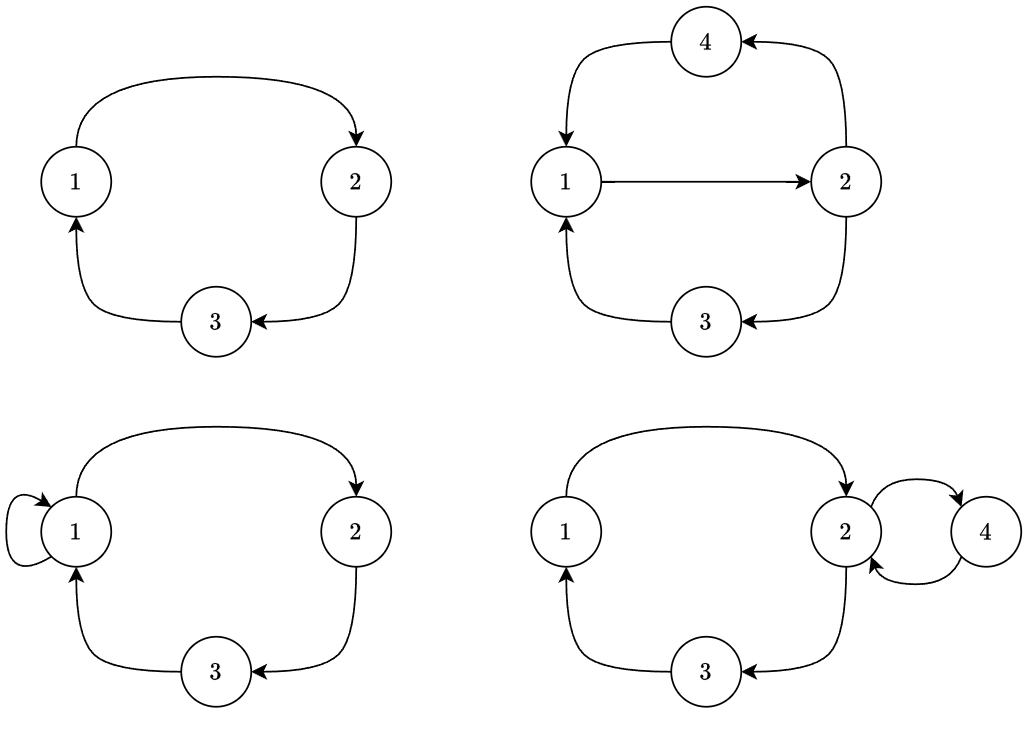
\includegraphics[width=0.5\linewidth]{images/period.png}
    \end{figure}
    Two are periodic, and the other two (bottom ones) are aperiodic.

    Consider the Markov chain described by the following transition matrix:
    \[P= 
    \begin{bmatrix}
        0.3 & 0.7 & 0 \\
        0.5 & 0 & 0.5 \\ 
        0 & 0.25 & 0.75
    \end{bmatrix}\]
    The corresponding graph is: 
    \begin{figure}[H]
        \centering
        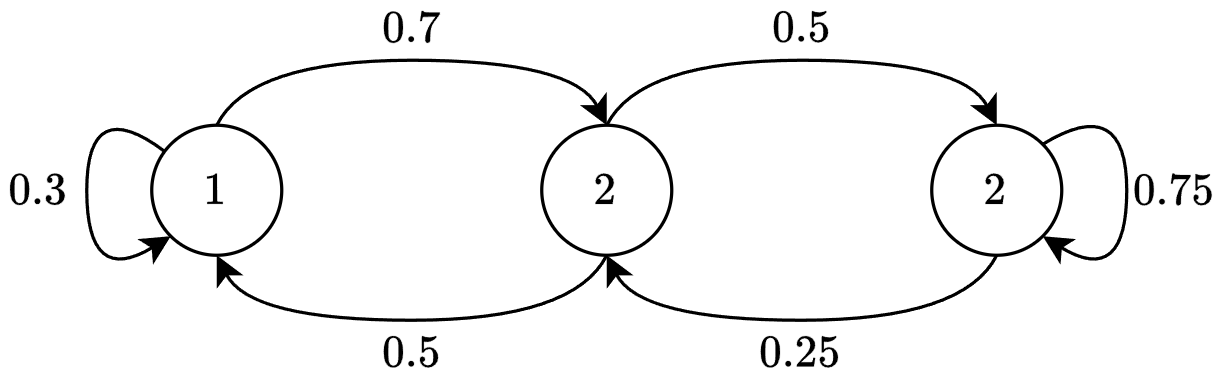
\includegraphics[width=0.5\linewidth]{images/ergo.png}
    \end{figure}
    We can see that this Markov chain is ergodic because it satisfies all the properties given in the definition.
\end{example}

\paragraph*{Steady state distribution}
Being $P$ the transition matrix of an ergodic Markov chain with $N$ states, we have that:
\[\lim_{n \rightarrow \infty}\Pr_{ij}(n)=\pi_j\]
With $\pi=\left[ \pi_1,\pi_2,\dots,\pi_N \right]$ being the steady-state distribution.

The behavior of a Markov chain before getting to the steady state is defined as transitory; we can compute the expected number of transitions to reach state $j$ being in state $i$ for an ergodic Markov chain as:
\[m_{ij}=p_{ij}(1)+\sum_{k \neq j}p_{ik}(1+m_{kj})=1+\sum_{k \neq j}p_{ik}\cdot m_{kj}\]
\begin{example}
    It is possible to compute how many bottles on average a Cola1 buyer will have before switching to Cola2:
    \[m_{12}=1+\sum_{k \neq j}p_{1k}\cdot m_{k2}=1+p_{11}\cdot m_{12}=1+0.9\cdot m_{12}=\dfrac{1}{1-0.9}=10\]
    And also how many bottles on average a Cola2 buyer will have before switching to Cola1:
    \[m_{21}=1+\sum_{k \neq j}p_{2k}\cdot m_{k1}=1+p_{22}\cdot m_{21}=1+0.8\cdot m_{21}=\dfrac{1}{1-0.8}=5\]
\end{example}

\paragraph*{Absorbing states}
We have an absorbing Markov chain if there exist one or more absorbing states and all the others are transient.
Its transition matrix is:
\[P=
\begin{bmatrix}
    Q & R \\
    0 & 1
\end{bmatrix}\]
Here, $Q$ is the transition matrix for transient states, and $R$ is the transition matrix from transient to absorbing states.

The average time spent in a transient state $j$, starting from a transient state $j$, is equal to the $ij$-th element of:
\[(I-Q)^{-1}\]

The probability to reach an absorbing state $ij$, starting from a transient state $i$, is equal to the $ij$-th element of: 
\[(I-Q)^{-1} \cdot R\]
\begin{example}
    Consider a company with three hierarchical levels: junior, senior, and partner. 
    At any time, a person could leave the company as a senior or not. 
    We can define a transition matrix with five columns: junior, senior, partner, leave not partner, and leave partner. 
    The matrix is the following:
    \[P= 
    \begin{bmatrix}
        0.80    & 0.15  & 0     & 0.05  & 0 \\
        0       & 0.70  & 0.20  & 0.10  & 0 \\
        0       & 0     & 0.95  & 0     & 0.05 \\
        0       & 0     & 0     & 1     & 0 \\
        0       & 0     & 0     & 0     & 1 \\
    \end{bmatrix}\]
    It is possible to separate the matrix into the four parts seen before.
    The average time spent in a transient state is:
    \[\textnormal{transient}=(I-Q)^{-1}=\left(  
        \begin{bmatrix}
            1       & 0     & 0  \\
            0       & 1     & 0  \\
            0       & 0     & 1  \\
        \end{bmatrix}
        \begin{bmatrix}
            0.80    & 0.15  & 0     \\
            0       & 0.70  & 0.20  \\
            0       & 0     & 0.95  \\
        \end{bmatrix}\right)^{-1}=        
    \begin{bmatrix}
        5       & 2.5   & 10    \\
        0       & 3.3   & 13.3  \\
        0       & 0     & 20    \\
    \end{bmatrix}\]
    We can compute how long a junior will remain in the company:
    \begin{itemize}
        \item As a junior: $m_{11}=5$.
        \item As a senior: $m_{12}=2.5$.
        \item As a partner: $m_{13}=10$.
    \end{itemize}
    With a total of 17.5 years.

    The probability to reach an absorbing state is:
    \[\textnormal{absorbing}=(I-Q)^{-1}R=
    \left(  
        \begin{bmatrix}
            1       & 0     & 0  \\
            0       & 1     & 0  \\
            0       & 0     & 1  \\
        \end{bmatrix}
        \begin{bmatrix}
            0.80    & 0.15  & 0     \\
            0       & 0.70  & 0.20  \\
            0       & 0     & 0.95  \\
        \end{bmatrix}
    \right)^{-1}
    \begin{bmatrix}
        0.05    & 0     \\
        0.10    & 0     \\
        0       & 0.05  \\
    \end{bmatrix}
    =        
    \begin{bmatrix}
        0.5     & 0.5   \\
        0.3     & 0.7   \\
        0       & 1     \\
    \end{bmatrix}\]
    The probability for a junior to leave the company as a partner is given by the $m_{12}$ element of the previous matrix, which has a value of 0.5.
\end{example}